\documentclass[oneside,final]{amsart}  % Add final option when final
\title{Math 5344 - Programming Problem 3}
\author{Nicholas Moore}
\usepackage{amsmath}
\usepackage{amssymb}
\usepackage{graphicx}
\usepackage{caption}
\usepackage{algorithm}
\usepackage{algpseudocode}
\usepackage{mathtools}
\usepackage{listings}
\usepackage{xcolor}
\usepackage[top=1in,bottom=1in,includefoot]{geometry}
\usepackage[
pdfauthor={Nicholas Moore},
pdftitle ={Math 5344 - Programming Problem 3},
pdfkeywords={},
pdfstartview={FitH},
bookmarks={true},
draft={false}   % Change this when final
]{hyperref}

\newenvironment{myproof}[1][\proofname]{\proof[#1]\mbox{}\\*}{\endproof}
\newcommand{\sign}{\mathrm{sign}}
\newcommand{\norm}[1]{\left\lVert #1 \right\rVert}

% New commands for -=, +=, *=, /=
\newcommand{\pluseq}{\mathrel{+}=}
\newcommand{\minuseq}{\mathrel{-}=}
\newcommand{\timeseq}{\mathrel{*}=}
\newcommand{\divideeq}{\mathrel{/}=}
\newcommand{\inv}{^{-1}}

\parskip 12pt           % sets spacing between paragraphs
% \renewcommand{\baselinestretch}{1.5} 	% Uncomment for 1.5 spacing between lines
% \renewcommand{\baselinestretch}{2.0}
\parindent 0pt		  % sets leading space for paragraphs

\allowdisplaybreaks[1]

% Colors and styles for typesetting Python code
\definecolor{codegreen}{rgb}{0,0.6,0}
\definecolor{codegray}{rgb}{0.5,0.5,0.5}
\definecolor{codepurple}{rgb}{0.58,0,0.82}
\definecolor{backcolour}{rgb}{0.95,0.95,0.92}

\lstdefinestyle{mystyle}{
  backgroundcolor=\color{backcolour},   
  commentstyle=\color{codegreen},
  keywordstyle=\color{magenta},
  numberstyle=\tiny\color{codegray},
  stringstyle=\color{codepurple},
  basicstyle=\ttfamily\footnotesize,
  breakatwhitespace=false,         
  breaklines=true,                 
  captionpos=b,                    
  keepspaces=true,                 
  numbers=left,                    
  numbersep=5pt,                  
  showspaces=false,                
  showstringspaces=false,
  showtabs=false,                  
  tabsize=2
}

\lstset{style=mystyle}

\begin{document}
\maketitle
\section{System Information}
  \begin{table}[htpb]
    \centering
    \begin{tabular}{|c|c|c|c|}
      \hline
      \multicolumn{4}{|c|}{\textbf{System: }Nick Moore's Desktop ``NickArch'' }\\
      \hline
      \hline
      \multicolumn{4}{|c|}{\textbf{Software}} \\
      \hline
      \textbf{OS} & \textbf{Python version} & \textbf{Numpy version} & \textbf{SciPy version} \\
      \hline
      Arch Linux (Kernel 5.9.9) & 3.8.6 & 1.19.4 & 1.5.4 \\
      \hline
      \multicolumn{4}{|c|}{\textbf{Processor Information}} \\
      \hline
      \multicolumn{2}{|c|}{\textbf{Processor}} & \textbf{Number of Cores} & \textbf{Speed} \\
      \hline
      \multicolumn{2}{|c|}{AMD Ryzen 7 3800X} & 8 (16 Threads) & 3.9GHz Base, Boost to 4.5GHz \\
      \hline
      \multicolumn{4}{|c|}{\textbf{Memory Information}} \\
      \hline
      \multicolumn{2}{|c|}{\textbf{Main RAM}} & \textbf{L2} & \textbf{L3} \\
      \hline
      \multicolumn{2}{|c|}{32 GB @ 3000MHz DDR4} & 512KB  per core & 32MB \\
      \hline
    \end{tabular}
  \end{table}
\section{Results from DH CG}

Almost all runs of PCG with a drop tolerance or 1 and 0.1 did not converge, even
after 1000000 iterations, so those results are omitted.  The maximum CG iterations allowed for the
following results was 10000.

\begin{tabular}{|c|c|c|c|c|c|c|c|c|c|}
\hline
\multicolumn{10}{|c|}{Matrix: Debye-Huckel \#9}\tabularnewline
\hline
\multicolumn{10}{|l|}{Size: $289\times289$}\tabularnewline
\hline
\multicolumn{10}{|l|}{Solver: PCG}\tabularnewline
\hline
\multicolumn{10}{|l|}{Preconditioning: ILU right, \texttt{fill\_factor=30}}\tabularnewline
\hline
\hline
\multicolumn{10}{|c|}{Stopping tolerance: $\tau=10^{-6}$}\tabularnewline
\hline
\hline
 & \multicolumn{3}{c|}{Convergence} & \multicolumn{3}{c|}{Iterative solve time} & \multicolumn{3}{c|}{Direct solve}\tabularnewline
\hline
Fill drop tol.  & Iters & $\left\Vert r_{\text{final}}\right\Vert $  & $\left\Vert e\right\Vert $  & Build ILU  & PCG  & total  & $\left\Vert r\right\Vert $ & $\left\Vert e\right\Vert $  & time\tabularnewline
\hline
% Please table data here - 1e-06 tolerance
  0.01 & 11 & 2.72e-07 & 5.65e-06 &   0.000807 &   0.000713 &    0.00152 & 3.62e-16 & 1.38e-14 &   0.000812\\
  \hline
  0.001 & 3 & 4.10e-07 & 6.11e-06 &   0.000862 &   0.000247 &    0.00111 & 3.62e-16 & 1.38e-14 &   0.000812\\
  \hline
  0.0001 & 2 & 4.36e-07 & 2.77e-06 &   0.000829 &   0.000188 &    0.00102 & 3.62e-16 & 1.38e-14 &   0.000812\\
  \hline
\hline
\multicolumn{10}{|c|}{Stopping tolerance: $\tau=10^{-8}$}\tabularnewline
\hline
\hline
 & \multicolumn{3}{c|}{Convergence} & \multicolumn{3}{c|}{Iterative solve time} & \multicolumn{3}{c|}{Direct solve }\tabularnewline
\hline
Fill drop tol.  & Iters  & $\left\Vert r_{\text{final}}\right\Vert $  & $\left\Vert e\right\Vert $ & Build ILU  & PCG  & total  & $\left\Vert r\right\Vert $  & $\left\Vert e\right\Vert $  & time\tabularnewline
\hline
% Place table data here - 1e-08 tolerance
  0.01 & 15 & 3.38e-09 & 1.42e-08 &   0.000825 &    0.00087 &     0.0017 & 3.62e-16 & 1.38e-14 &   0.000812\\
  \hline
  0.001 & 4 & 5.81e-09 & 3.75e-08 &    0.00082 &   0.000306 &    0.00113 & 3.62e-16 & 1.38e-14 &   0.000812\\
  \hline
  0.0001 & 3 & 1.83e-10 & 5.79e-09 &   0.000815 &   0.000244 &    0.00106 & 3.62e-16 & 1.38e-14 &   0.000812\\
  \hline
\end{tabular}

\begin{tabular}{|c|c|c|c|c|c|c|c|c|c|}
\hline
\multicolumn{10}{|c|}{Matrix: Debye-Huckel \#10}\tabularnewline
\hline
  \multicolumn{10}{|l|}{Size: $545\times545$}\tabularnewline
\hline
\multicolumn{10}{|l|}{Solver: PCG}\tabularnewline
\hline
\multicolumn{10}{|l|}{Preconditioning: ILU right, \texttt{fill\_factor=30}}\tabularnewline
\hline
\hline
\multicolumn{10}{|c|}{Stopping tolerance: $\tau=10^{-6}$}\tabularnewline
\hline
\hline
 & \multicolumn{3}{c|}{Convergence} & \multicolumn{3}{c|}{Iterative solve time} & \multicolumn{3}{c|}{Direct solve}\tabularnewline
\hline
Fill drop tol.  & Iters & $\left\Vert r_{\text{final}}\right\Vert $  & $\left\Vert e\right\Vert $  & Build ILU  & PCG  & total  & $\left\Vert r\right\Vert $ & $\left\Vert e\right\Vert $  & time\tabularnewline
\hline
% Please table data here - 1e-06 tolerance
  0.01 & 12 & 5.94e-07 & 2.77e-05 &    0.00163 &    0.00151 &    0.00314 & 3.46e-16 & 2.95e-14 &    0.00151\\
  \hline
  0.001 & 4 & 1.58e-07 & 4.11e-06 &    0.00167 &    0.00064 &    0.00231 & 3.46e-16 & 2.95e-14 &    0.00151\\
  \hline
  0.0001 & 2 & 3.46e-07 & 1.28e-06 &    0.00165 &   0.000384 &    0.00204 & 3.46e-16 & 2.95e-14 &    0.00151\\
  \hline
\hline
\multicolumn{10}{|c|}{Stopping tolerance: $\tau=10^{-8}$}\tabularnewline
\hline
\hline
 & \multicolumn{3}{c|}{Convergence} & \multicolumn{3}{c|}{Iterative solve time} & \multicolumn{3}{c|}{Direct solve }\tabularnewline
\hline
Fill drop tol.  & Iters  & $\left\Vert r_{\text{final}}\right\Vert $  & $\left\Vert e\right\Vert $ & Build ILU  & PCG  & total  & $\left\Vert r\right\Vert $  & $\left\Vert e\right\Vert $  & time\tabularnewline
\hline
% Place table data here - 1e-08 tolerance
  0.01 & 18 & 7.29e-09 & 5.08e-07 &    0.00164 &     0.0022 &    0.00384 & 3.46e-16 & 2.95e-14 &    0.00151\\
  \hline
  0.001 & 5 & 2.62e-09 & 9.71e-09 &    0.00123 &    0.00049 &    0.00172 & 3.46e-16 & 2.95e-14 &    0.00151\\
  \hline
  0.0001 & 3 & 5.21e-11 & 2.52e-09 &    0.00121 &   0.000341 &    0.00155 & 3.46e-16 & 2.95e-14 &    0.00151\\
  \hline
\end{tabular}

\begin{tabular}{|c|c|c|c|c|c|c|c|c|c|}
\hline
\multicolumn{10}{|c|}{Matrix: Debye-Huckel \#11}\tabularnewline
\hline
  \multicolumn{10}{|l|}{Size: $1089\times1089$}\tabularnewline
\hline
\multicolumn{10}{|l|}{Solver: PCG}\tabularnewline
\hline
\multicolumn{10}{|l|}{Preconditioning: ILU right, \texttt{fill\_factor=30}}\tabularnewline
\hline
\hline
\multicolumn{10}{|c|}{Stopping tolerance: $\tau=10^{-6}$}\tabularnewline
\hline
\hline
 & \multicolumn{3}{c|}{Convergence} & \multicolumn{3}{c|}{Iterative solve time} & \multicolumn{3}{c|}{Direct solve}\tabularnewline
\hline
Fill drop tol.  & Iters & $\left\Vert r_{\text{final}}\right\Vert $  & $\left\Vert e\right\Vert $  & Build ILU  & PCG  & total  & $\left\Vert r\right\Vert $ & $\left\Vert e\right\Vert $  & time\tabularnewline
\hline
% Please table data here - 1e-06 tolerance
  0.01 & 24 & 5.62e-07 & 1.34e-04 &    0.00259 &    0.00246 &    0.00505 & 3.64e-16 & 8.78e-15 &    0.00244\\
  \hline
  0.001 & 6 & 7.22e-08 & 1.86e-05 &     0.0028 &   0.000788 &    0.00359 & 3.64e-16 & 8.78e-15 &    0.00244\\
  \hline
  0.0001 & 2 & 2.14e-07 & 2.90e-06 &     0.0028 &   0.000364 &    0.00317 & 3.64e-16 & 8.78e-15 &    0.00244\\
  \hline
\hline
\multicolumn{10}{|c|}{Stopping tolerance: $\tau=10^{-8}$}\tabularnewline
\hline
\hline
 & \multicolumn{3}{c|}{Convergence} & \multicolumn{3}{c|}{Iterative solve time} & \multicolumn{3}{c|}{Direct solve }\tabularnewline
\hline
Fill drop tol.  & Iters  & $\left\Vert r_{\text{final}}\right\Vert $  & $\left\Vert e\right\Vert $ & Build ILU  & PCG  & total  & $\left\Vert r\right\Vert $  & $\left\Vert e\right\Vert $  & time\tabularnewline
\hline
% Place table data here - 1e-08 tolerance
  0.01 & 40 & 3.70e-09 & 7.75e-07 &    0.00263 &    0.00395 &    0.00659 & 3.64e-16 & 8.78e-15 &    0.00244\\
  \hline
  0.001 & 9 & 4.37e-09 & 4.25e-07 &    0.00277 &     0.0011 &    0.00387 & 3.64e-16 & 8.78e-15 &    0.00244\\
  \hline
  0.0001 & 3 & 1.74e-10 & 4.04e-09 &    0.00277 &   0.000466 &    0.00324 & 3.64e-16 & 8.78e-15 &    0.00244\\
  \hline
\end{tabular}

\begin{tabular}{|c|c|c|c|c|c|c|c|c|c|}
\hline
\multicolumn{10}{|c|}{Matrix: Debye-Huckel \#12}\tabularnewline
\hline
  \multicolumn{10}{|l|}{Size: $2113\times2113$}\tabularnewline
\hline
\multicolumn{10}{|l|}{Solver: PCG}\tabularnewline
\hline
\multicolumn{10}{|l|}{Preconditioning: ILU right, \texttt{fill\_factor=30}}\tabularnewline
\hline
\hline
\multicolumn{10}{|c|}{Stopping tolerance: $\tau=10^{-6}$}\tabularnewline
\hline
\hline
 & \multicolumn{3}{c|}{Convergence} & \multicolumn{3}{c|}{Iterative solve time} & \multicolumn{3}{c|}{Direct solve}\tabularnewline
\hline
Fill drop tol.  & Iters & $\left\Vert r_{\text{final}}\right\Vert $  & $\left\Vert e\right\Vert $  & Build ILU  & PCG  & total  & $\left\Vert r\right\Vert $ & $\left\Vert e\right\Vert $  & time\tabularnewline
\hline
% Please table data here - 1e-06 tolerance
  0.01 & 23 & 4.87e-07 & 7.60e-05 &    0.00585 &    0.00484 &     0.0107 & 3.89e-16 & 2.31e-14 &    0.00559\\
  \hline
  0.001 & 7 & 4.39e-07 & 5.61e-05 &     0.0066 &    0.00186 &    0.00846 & 3.89e-16 & 2.31e-14 &    0.00559\\
  \hline
  0.0001 & 3 & 3.07e-08 & 3.32e-06 &    0.00674 &   0.000998 &    0.00774 & 3.89e-16 & 2.31e-14 &    0.00559\\
  \hline
\hline
\multicolumn{10}{|c|}{Stopping tolerance: $\tau=10^{-8}$}\tabularnewline
\hline
\hline
 & \multicolumn{3}{c|}{Convergence} & \multicolumn{3}{c|}{Iterative solve time} & \multicolumn{3}{c|}{Direct solve }\tabularnewline
\hline
Fill drop tol.  & Iters  & $\left\Vert r_{\text{final}}\right\Vert $  & $\left\Vert e\right\Vert $ & Build ILU  & PCG  & total  & $\left\Vert r\right\Vert $  & $\left\Vert e\right\Vert $  & time\tabularnewline
\hline
% Place table data here - 1e-08 tolerance
  0.01 & 35 & 4.87e-09 & 1.02e-06 &    0.00588 &    0.00716 &      0.013 & 3.89e-16 & 2.31e-14 &    0.00559\\
  \hline
  0.001 & 11 & 1.67e-09 & 9.14e-07 &    0.00653 &    0.00275 &    0.00928 & 3.89e-16 & 2.31e-14 &    0.00559\\
  \hline
  0.0001 & 4 & 2.46e-09 & 9.65e-08 &    0.00675 &    0.00124 &    0.00799 & 3.89e-16 & 2.31e-14 &    0.00559\\
  \hline
\end{tabular}

\begin{tabular}{|c|c|c|c|c|c|c|c|c|c|}
\hline
\multicolumn{10}{|c|}{Matrix: Debye-Huckel \#13}\tabularnewline
\hline
  \multicolumn{10}{|l|}{Size: $4225\times4225$}\tabularnewline
\hline
\multicolumn{10}{|l|}{Solver: PCG}\tabularnewline
\hline
\multicolumn{10}{|l|}{Preconditioning: ILU right, \texttt{fill\_factor=30}}\tabularnewline
\hline
\hline
\multicolumn{10}{|c|}{Stopping tolerance: $\tau=10^{-6}$}\tabularnewline
\hline
\hline
 & \multicolumn{3}{c|}{Convergence} & \multicolumn{3}{c|}{Iterative solve time} & \multicolumn{3}{c|}{Direct solve}\tabularnewline
\hline
Fill drop tol.  & Iters & $\left\Vert r_{\text{final}}\right\Vert $  & $\left\Vert e\right\Vert $  & Build ILU  & PCG  & total  & $\left\Vert r\right\Vert $ & $\left\Vert e\right\Vert $  & time\tabularnewline
\hline
% Please table data here - 1e-06 tolerance
  0.01 & 32 & 9.08e-07 & 3.52e-05 &     0.0123 &     0.0117 &      0.024 & 4.24e-16 & 1.01e-13 &     0.0122\\
  \hline
  0.001 & 10 & 1.85e-07 & 4.40e-06 &     0.0145 &    0.00452 &      0.019 & 4.24e-16 & 1.01e-13 &     0.0122\\
  \hline
  0.0001 & 3 & 4.91e-07 & 2.60e-05 &     0.0153 &     0.0018 &     0.0171 & 4.24e-16 & 1.01e-13 &     0.0122\\
  \hline
\hline
\multicolumn{10}{|c|}{Stopping tolerance: $\tau=10^{-8}$}\tabularnewline
\hline
\hline
 & \multicolumn{3}{c|}{Convergence} & \multicolumn{3}{c|}{Iterative solve time} & \multicolumn{3}{c|}{Direct solve }\tabularnewline
\hline
Fill drop tol.  & Iters  & $\left\Vert r_{\text{final}}\right\Vert $  & $\left\Vert e\right\Vert $ & Build ILU  & PCG  & total  & $\left\Vert r\right\Vert $  & $\left\Vert e\right\Vert $  & time\tabularnewline
\hline
% Place table data here - 1e-08 tolerance
  0.01 & 52 & 7.57e-09 & 1.60e-07 &     0.0125 &     0.0187 &     0.0312 & 4.24e-16 & 1.01e-13 &     0.0122\\
  \hline
  0.001 & 12 & 9.36e-09 & 2.70e-06 &     0.0144 &    0.00534 &     0.0197 & 4.24e-16 & 1.01e-13 &     0.0122\\
  \hline
  0.0001 & 5 & 5.33e-09 & 1.68e-07 &     0.0153 &    0.00267 &      0.018 & 4.24e-16 & 1.01e-13 &     0.0122\\
  \hline
\end{tabular}

\begin{tabular}{|c|c|c|c|c|c|c|c|c|c|}
\hline
\multicolumn{10}{|c|}{Matrix: Debye-Huckel \#14}\tabularnewline
\hline
  \multicolumn{10}{|l|}{Size: $8321\times8321$}\tabularnewline
\hline
\multicolumn{10}{|l|}{Solver: PCG}\tabularnewline
\hline
\multicolumn{10}{|l|}{Preconditioning: ILU right, \texttt{fill\_factor=30}}\tabularnewline
\hline
\hline
\multicolumn{10}{|c|}{Stopping tolerance: $\tau=10^{-6}$}\tabularnewline
\hline
\hline
 & \multicolumn{3}{c|}{Convergence} & \multicolumn{3}{c|}{Iterative solve time} & \multicolumn{3}{c|}{Direct solve}\tabularnewline
\hline
Fill drop tol.  & Iters & $\left\Vert r_{\text{final}}\right\Vert $  & $\left\Vert e\right\Vert $  & Build ILU  & PCG  & total  & $\left\Vert r\right\Vert $ & $\left\Vert e\right\Vert $  & time\tabularnewline
\hline
% Please table data here - 1e-06 tolerance
  0.01 & 31 & 5.81e-07 & 6.90e-04 &      0.039 &     0.0328 &     0.0717 & 4.44e-16 & 1.43e-13 &     0.0361\\
  \hline
  0.001 & 13 & 7.92e-07 & 2.47e-05 &     0.0358 &     0.0121 &     0.0479 & 4.44e-16 & 1.43e-13 &     0.0361\\
  \hline
  0.0001 & 4 & 2.79e-07 & 3.19e-04 &     0.0403 &    0.00487 &     0.0452 & 4.44e-16 & 1.43e-13 &     0.0361\\
  \hline
\hline
\multicolumn{10}{|c|}{Stopping tolerance: $\tau=10^{-8}$}\tabularnewline
\hline
\hline
 & \multicolumn{3}{c|}{Convergence} & \multicolumn{3}{c|}{Iterative solve time} & \multicolumn{3}{c|}{Direct solve }\tabularnewline
\hline
Fill drop tol.  & Iters  & $\left\Vert r_{\text{final}}\right\Vert $  & $\left\Vert e\right\Vert $ & Build ILU  & PCG  & total  & $\left\Vert r\right\Vert $  & $\left\Vert e\right\Vert $  & time\tabularnewline
\hline
% Place table data here - 1e-08 tolerance
  0.01 & 59 & 5.32e-09 & 1.26e-06 &     0.0281 &     0.0433 &     0.0715 & 4.44e-16 & 1.43e-13 &     0.0361\\
  \hline
  0.001 & 21 & 1.80e-09 & 1.82e-07 &      0.035 &     0.0183 &     0.0532 & 4.44e-16 & 1.43e-13 &     0.0361\\
  \hline
  0.0001 & 6 & 5.56e-09 & 4.82e-07 &     0.0395 &    0.00681 &     0.0463 & 4.44e-16 & 1.43e-13 &     0.0361\\
  \hline
\end{tabular}

\begin{tabular}{|c|c|c|c|c|c|c|c|c|c|}
\hline
\multicolumn{10}{|c|}{Matrix: Debye-Huckel \#15}\tabularnewline
\hline
  \multicolumn{10}{|l|}{Size: $16641\times16641$}\tabularnewline
\hline
\multicolumn{10}{|l|}{Solver: PCG}\tabularnewline
\hline
\multicolumn{10}{|l|}{Preconditioning: ILU right, \texttt{fill\_factor=30}}\tabularnewline
\hline
\hline
\multicolumn{10}{|c|}{Stopping tolerance: $\tau=10^{-6}$}\tabularnewline
\hline
\hline
 & \multicolumn{3}{c|}{Convergence} & \multicolumn{3}{c|}{Iterative solve time} & \multicolumn{3}{c|}{Direct solve}\tabularnewline
\hline
Fill drop tol.  & Iters & $\left\Vert r_{\text{final}}\right\Vert $  & $\left\Vert e\right\Vert $  & Build ILU  & PCG  & total  & $\left\Vert r\right\Vert $ & $\left\Vert e\right\Vert $  & time\tabularnewline
\hline
% Please table data here - 1e-06 tolerance
  0.01 & 44 & 7.06e-07 & 1.23e-03 &     0.0825 &     0.0769 &      0.159 & 4.77e-16 & 9.31e-14 &      0.105\\
  \hline
  0.001 & 13 & 5.73e-07 & 1.55e-03 &     0.0802 &     0.0292 &      0.109 & 4.77e-16 & 9.31e-14 &      0.105\\
  \hline
  0.0001 & 7 & 8.82e-08 & 1.77e-05 &     0.0961 &     0.0213 &      0.117 & 4.77e-16 & 9.31e-14 &      0.105\\
  \hline
\hline
\multicolumn{10}{|c|}{Stopping tolerance: $\tau=10^{-8}$}\tabularnewline
\hline
\hline
 & \multicolumn{3}{c|}{Convergence} & \multicolumn{3}{c|}{Iterative solve time} & \multicolumn{3}{c|}{Direct solve }\tabularnewline
\hline
Fill drop tol.  & Iters  & $\left\Vert r_{\text{final}}\right\Vert $  & $\left\Vert e\right\Vert $ & Build ILU  & PCG  & total  & $\left\Vert r\right\Vert $  & $\left\Vert e\right\Vert $  & time\tabularnewline
\hline
% Place table data here - 1e-08 tolerance
  0.01 & 84 & 8.36e-09 & 7.80e-06 &     0.0641 &      0.146 &       0.21 & 4.77e-16 & 9.31e-14 &      0.105\\
  \hline
  0.001 & 22 & 4.80e-09 & 4.07e-06 &     0.0802 &     0.0471 &      0.127 & 4.77e-16 & 9.31e-14 &      0.105\\
  \hline
  0.0001 & 8 & 9.20e-09 & 1.32e-05 &     0.0957 &     0.0271 &      0.123 & 4.77e-16 & 9.31e-14 &      0.105\\
  \hline
\end{tabular}

\begin{tabular}{|c|c|c|c|c|c|c|c|c|c|}
\hline
\multicolumn{10}{|c|}{Matrix: Debye-Huckel \#16}\tabularnewline
\hline
  \multicolumn{10}{|l|}{Size: $65137\times65137$}\tabularnewline
\hline
\multicolumn{10}{|l|}{Solver: PCG}\tabularnewline
\hline
\multicolumn{10}{|l|}{Preconditioning: ILU right, \texttt{fill\_factor=30}}\tabularnewline
\hline
\hline
\multicolumn{10}{|c|}{Stopping tolerance: $\tau=10^{-6}$}\tabularnewline
\hline
\hline
 & \multicolumn{3}{c|}{Convergence} & \multicolumn{3}{c|}{Iterative solve time} & \multicolumn{3}{c|}{Direct solve}\tabularnewline
\hline
Fill drop tol.  & Iters & $\left\Vert r_{\text{final}}\right\Vert $  & $\left\Vert e\right\Vert $  & Build ILU  & PCG  & total  & $\left\Vert r\right\Vert $ & $\left\Vert e\right\Vert $  & time\tabularnewline
\hline
% Please table data here - 1e-06 tolerance
  0.01 & 82 & 9.89e-07 & 1.37e-03 &      0.295 &      0.561 &      0.855 & 5.40e-16 & 6.52e-13 &      0.808\\
  \hline
  0.001 & 23 & 8.00e-07 & 1.10e-03 &      0.385 &      0.248 &      0.633 & 5.40e-16 & 6.52e-13 &      0.808\\
  \hline
  0.0001 & 11 & 2.32e-07 & 8.00e-05 &      0.514 &      0.171 &      0.685 & 5.40e-16 & 6.52e-13 &      0.808\\
  \hline
\hline
\multicolumn{10}{|c|}{Stopping tolerance: $\tau=10^{-8}$}\tabularnewline
\hline
\hline
 & \multicolumn{3}{c|}{Convergence} & \multicolumn{3}{c|}{Iterative solve time} & \multicolumn{3}{c|}{Direct solve }\tabularnewline
\hline
Fill drop tol.  & Iters  & $\left\Vert r_{\text{final}}\right\Vert $  & $\left\Vert e\right\Vert $ & Build ILU  & PCG  & total  & $\left\Vert r\right\Vert $  & $\left\Vert e\right\Vert $  & time\tabularnewline
\hline
% Place table data here - 1e-08 tolerance
  0.01 & 257 & 9.79e-09 & 1.24e-05 &      0.283 &       1.75 &       2.03 & 5.40e-16 & 6.52e-13 &      0.808\\
  \hline
  0.001 & 39 & 5.42e-09 & 3.20e-06 &       0.38 &      0.423 &      0.802 & 5.40e-16 & 6.52e-13 &      0.808\\
  \hline
  0.0001 & 14 & 6.78e-09 & 1.01e-05 &      0.503 &      0.208 &      0.711 & 5.40e-16 & 6.52e-13 &      0.808\\
  \hline
\end{tabular}

\begin{tabular}{|c|c|c|c|c|c|c|c|c|c|}
\hline
\multicolumn{10}{|c|}{Matrix: Debye-Huckel \#17}\tabularnewline
\hline
  \multicolumn{10}{|l|}{Size: $95538\times95538$}\tabularnewline
\hline
\multicolumn{10}{|l|}{Solver: PCG}\tabularnewline
\hline
\multicolumn{10}{|l|}{Preconditioning: ILU right, \texttt{fill\_factor=30}}\tabularnewline
\hline
\hline
\multicolumn{10}{|c|}{Stopping tolerance: $\tau=10^{-6}$}\tabularnewline
\hline
\hline
 & \multicolumn{3}{c|}{Convergence} & \multicolumn{3}{c|}{Iterative solve time} & \multicolumn{3}{c|}{Direct solve}\tabularnewline
\hline
Fill drop tol.  & Iters & $\left\Vert r_{\text{final}}\right\Vert $  & $\left\Vert e\right\Vert $  & Build ILU  & PCG  & total  & $\left\Vert r\right\Vert $ & $\left\Vert e\right\Vert $  & time\tabularnewline
\hline
% Please table data here - 1e-06 tolerance
  0.01 & 109 & 9.99e-07 & 9.32e-04 &      0.497 &        1.2 &        1.7 & 5.23e-16 & 5.62e-13 &       1.39\\
  \hline
  0.001 & 26 & 8.79e-07 & 4.20e-04 &      0.643 &      0.416 &       1.06 & 5.23e-16 & 5.62e-13 &       1.39\\
  \hline
  0.0001 & 13 & 4.27e-07 & 2.00e-04 &       0.85 &      0.277 &       1.13 & 5.23e-16 & 5.62e-13 &       1.39\\
  \hline
\hline
\multicolumn{10}{|c|}{Stopping tolerance: $\tau=10^{-8}$}\tabularnewline
\hline
\hline
 & \multicolumn{3}{c|}{Convergence} & \multicolumn{3}{c|}{Iterative solve time} & \multicolumn{3}{c|}{Direct solve }\tabularnewline
\hline
Fill drop tol.  & Iters  & $\left\Vert r_{\text{final}}\right\Vert $  & $\left\Vert e\right\Vert $ & Build ILU  & PCG  & total  & $\left\Vert r\right\Vert $  & $\left\Vert e\right\Vert $  & time\tabularnewline
\hline
% Place table data here - 1e-08 tolerance
  0.01 & 498 & 9.89e-09 & 1.44e-05 &       0.49 &       5.47 &       5.96 & 5.23e-16 & 5.62e-13 &       1.39\\
  \hline
  0.001 & 47 & 8.99e-09 & 1.61e-06 &      0.641 &      0.745 &       1.39 & 5.23e-16 & 5.62e-13 &       1.39\\
  \hline
  0.0001 & 21 & 7.25e-09 & 2.21e-06 &      0.848 &      0.462 &       1.31 & 5.23e-16 & 5.62e-13 &       1.39\\
  \hline
\end{tabular}

\begin{tabular}{|c|c|c|c|c|c|c|c|c|c|}
\hline
\multicolumn{10}{|c|}{Matrix: Debye-Huckel \#18}\tabularnewline
\hline
  \multicolumn{10}{|l|}{Size: $197830\times197830$}\tabularnewline
\hline
\multicolumn{10}{|l|}{Solver: PCG}\tabularnewline
\hline
\multicolumn{10}{|l|}{Preconditioning: ILU right, \texttt{fill\_factor=30}}\tabularnewline
\hline
\hline
\multicolumn{10}{|c|}{Stopping tolerance: $\tau=10^{-6}$}\tabularnewline
\hline
\hline
 & \multicolumn{3}{c|}{Convergence} & \multicolumn{3}{c|}{Iterative solve time} & \multicolumn{3}{c|}{Direct solve}\tabularnewline
\hline
Fill drop tol.  & Iters & $\left\Vert r_{\text{final}}\right\Vert $  & $\left\Vert e\right\Vert $  & Build ILU  & PCG  & total  & $\left\Vert r\right\Vert $ & $\left\Vert e\right\Vert $  & time\tabularnewline
\hline
% Please table data here - 1e-06 tolerance
  0.01 & 140 & 9.93e-07 & 1.34e-03 &       1.21 &       3.22 &       4.43 & 6.15e-16 & 2.09e-12 &        5.2\\
  \hline
  0.001 & 41 & 9.30e-07 & 3.11e-04 &       1.66 &       1.47 &       3.13 & 6.15e-16 & 2.09e-12 &        5.2\\
  \hline
  0.0001 & 14 & 5.58e-07 & 4.47e-03 &       2.52 &      0.719 &       3.24 & 6.15e-16 & 2.09e-12 &        5.2\\
  \hline
\hline
\multicolumn{10}{|c|}{Stopping tolerance: $\tau=10^{-8}$}\tabularnewline
\hline
\hline
 & \multicolumn{3}{c|}{Convergence} & \multicolumn{3}{c|}{Iterative solve time} & \multicolumn{3}{c|}{Direct solve }\tabularnewline
\hline
Fill drop tol.  & Iters  & $\left\Vert r_{\text{final}}\right\Vert $  & $\left\Vert e\right\Vert $ & Build ILU  & PCG  & total  & $\left\Vert r\right\Vert $  & $\left\Vert e\right\Vert $  & time\tabularnewline
\hline
% Place table data here - 1e-08 tolerance
  0.01 & 10000 & 2.51e-08 & 1.35e-05 &       1.21 &        227 &        228 & 6.15e-16 & 2.09e-12 &        5.2\\
  \hline
  0.001 & 52 & 8.52e-09 & 5.74e-05 &       1.64 &       1.84 &       3.48 & 6.15e-16 & 2.09e-12 &        5.2\\
  \hline
  0.0001 & 25 & 9.67e-09 & 5.25e-05 &       2.49 &       1.22 &       3.71 & 6.15e-16 & 2.09e-12 &        5.2\\
  \hline
\end{tabular}

\begin{tabular}{|c|c|c|c|c|c|c|c|c|c|}
\hline
\multicolumn{10}{|c|}{Matrix: Debye-Huckel \#19}\tabularnewline
\hline
  \multicolumn{10}{|l|}{Size: $436218\times436218$}\tabularnewline
\hline
\multicolumn{10}{|l|}{Solver: PCG}\tabularnewline
\hline
\multicolumn{10}{|l|}{Preconditioning: ILU right, \texttt{fill\_factor=30}}\tabularnewline
\hline
\hline
\multicolumn{10}{|c|}{Stopping tolerance: $\tau=10^{-6}$}\tabularnewline
\hline
\hline
 & \multicolumn{3}{c|}{Convergence} & \multicolumn{3}{c|}{Iterative solve time} & \multicolumn{3}{c|}{Direct solve}\tabularnewline
\hline
Fill drop tol.  & Iters & $\left\Vert r_{\text{final}}\right\Vert $  & $\left\Vert e\right\Vert $  & Build ILU  & PCG  & total  & $\left\Vert r\right\Vert $ & $\left\Vert e\right\Vert $  & time\tabularnewline
\hline
% Please table data here - 1e-06 tolerance
  0.01 & 252 & 9.89e-07 & 1.41e-03 &       2.83 &         13 &       15.8 & 5.63e-16 & 5.46e-12 &       12.8\\
  \hline
  0.001 & 44 & 8.86e-07 & 1.19e-03 &       4.21 &       3.34 &       7.55 & 5.63e-16 & 5.46e-12 &       12.8\\
  \hline
  0.0001 & 18 & 5.56e-07 & 1.69e-03 &       7.09 &       1.87 &       8.96 & 5.63e-16 & 5.46e-12 &       12.8\\
  \hline
\hline
\multicolumn{10}{|c|}{Stopping tolerance: $\tau=10^{-8}$}\tabularnewline
\hline
\hline
 & \multicolumn{3}{c|}{Convergence} & \multicolumn{3}{c|}{Iterative solve time} & \multicolumn{3}{c|}{Direct solve }\tabularnewline
\hline
Fill drop tol.  & Iters  & $\left\Vert r_{\text{final}}\right\Vert $  & $\left\Vert e\right\Vert $ & Build ILU  & PCG  & total  & $\left\Vert r\right\Vert $  & $\left\Vert e\right\Vert $  & time\tabularnewline
\hline
% Place table data here - 1e-08 tolerance
  0.01 & 10000 & 4.18e-07 & 4.03e-05 &       2.81 &        514 &        517 & 5.63e-16 & 5.46e-12 &       12.8\\
  \hline
  0.001 & 94 & 9.32e-09 & 3.07e-06 &       4.21 &       7.03 &       11.2 & 5.63e-16 & 5.46e-12 &       12.8\\
  \hline
  0.0001 & 32 & 7.14e-09 & 4.73e-06 &       7.07 &       3.25 &       10.3 & 5.63e-16 & 5.46e-12 &       12.8\\
  \hline
\end{tabular}

\begin{tabular}{|c|c|c|c|c|c|c|c|c|c|}
\hline
\multicolumn{10}{|c|}{Matrix: Debye-Huckel \#20}\tabularnewline
\hline
  \multicolumn{10}{|l|}{Size: $769494\times769494$}\tabularnewline
\hline
\multicolumn{10}{|l|}{Solver: PCG}\tabularnewline
\hline
\multicolumn{10}{|l|}{Preconditioning: ILU right, \texttt{fill\_factor=30}}\tabularnewline
\hline
\hline
\multicolumn{10}{|c|}{Stopping tolerance: $\tau=10^{-6}$}\tabularnewline
\hline
\hline
 & \multicolumn{3}{c|}{Convergence} & \multicolumn{3}{c|}{Iterative solve time} & \multicolumn{3}{c|}{Direct solve}\tabularnewline
\hline
Fill drop tol.  & Iters & $\left\Vert r_{\text{final}}\right\Vert $  & $\left\Vert e\right\Vert $  & Build ILU  & PCG  & total  & $\left\Vert r\right\Vert $ & $\left\Vert e\right\Vert $  & time\tabularnewline
\hline
% Please table data here - 1e-06 tolerance
  0.01 & 411 & 9.96e-07 & 1.34e-03 &       6.22 &       39.3 &       45.5 & 6.46e-16 & 2.11e-11 &       42.6\\
  \hline
  0.001 & 56 & 8.35e-07 & 1.65e-03 &       10.8 &       7.96 &       18.7 & 6.46e-16 & 2.11e-11 &       42.6\\
  \hline
  0.0001 & 21 & 6.68e-07 & 2.21e-03 &       17.7 &        4.1 &       21.8 & 6.46e-16 & 2.11e-11 &       42.6\\
  \hline
\hline
\multicolumn{10}{|c|}{Stopping tolerance: $\tau=10^{-8}$}\tabularnewline
\hline
\hline
 & \multicolumn{3}{c|}{Convergence} & \multicolumn{3}{c|}{Iterative solve time} & \multicolumn{3}{c|}{Direct solve }\tabularnewline
\hline
Fill drop tol.  & Iters  & $\left\Vert r_{\text{final}}\right\Vert $  & $\left\Vert e\right\Vert $ & Build ILU  & PCG  & total  & $\left\Vert r\right\Vert $  & $\left\Vert e\right\Vert $  & time\tabularnewline
\hline
% Place table data here - 1e-08 tolerance
  0.01 & 10000 & 5.44e-07 & 6.05e-04 &       6.23 &        956 &        962 & 6.46e-16 & 2.11e-11 &       42.6\\
  \hline
  0.001 & 99 & 9.16e-09 & 1.92e-04 &       10.7 &       13.9 &       24.6 & 6.46e-16 & 2.11e-11 &       42.6\\
  \hline
  0.0001 & 39 & 9.68e-09 & 1.47e-05 &       17.6 &       7.37 &         25 & 6.46e-16 & 2.11e-11 &       42.6\\
  \hline
\end{tabular}

\section{Analysis}
Preconditioned CG with the correct drop tolerance appears to always achieve the desired accuracy in
a quicker time than the Direct Solve. It does depend on the drop tolerance. It should also be noted
that at the larger drop tolerances, 0.1 and 1, the CG method did not converge, even with a large
number of maximum iterations.  Also, we larger matrices, the performance of the 0.01 drop tolerance
also started to suffer.  In a couple of cases, the number of iterations required exceeded 10000,
leading to large timings.  The smaller drop tolerances however were very effective, often twice as
fast as the direct method, even for the larger matrices.

Even in larger sizes, the direct solver is still able to achieve a residual of around machine epsilon.
Even at high fill drop tolerance, the preconditioner performance is still improving, so there does
not appear to be any roundoff issues.

\section{Error Analysis}
The original problem called for calculating the condition number using \texttt{np.linalg.cond}, but
this function requires a dense matrix, severely limiting the capability to calculate the condition
number of the larger matrices.
Even on my machine with 32G of ram, matrix 16 was too large to fit.

As an alternative, we can use a spare function to approximate the largest and smallest eigenvalues
of a sparse matrix.  The code is given below:
\begin{lstlisting}[language=Python]
  import scipy.sparse.linalg as splu
  evl, _ = splu.eigs(A, which='LM')
  evs, _ = splu.eigs(A, sigma=1e-8)
  evl = abs(evl)
  evs = abs(evs)
  condNum = evl.max()/evs.min()
\end{lstlisting}
The \texttt{eigs} function uses the Implicitly Restarted Arnoldi Method to find eigenvalues and eigenvectors.
The \texttt{evl} finds the ``Largest Magnitude (LM)'' eigenvalue, while the \texttt{evs} finds the
eigenvalue closest to \texttt{sigma = 1e-8} using a shift-invert mode.  See the documentation at
\href{https://docs.scipy.org/doc/scipy/reference/generated/scipy.sparse.linalg.eigs.html}{this link} for more
information.

I tested this value against the value calculated from \texttt{np.linalg.cond} for matrices 6, 10,
12, and 14. The results were all within \texttt{1e-1} and calculated significantly faster as
well. Below I have included the condition numbers for selected matrices as well as the timing
information using the above code:
\begin{center}
\begin{tabular}{|c|c|c|}
  \hline
  Matrix & $\kappa$ & time (sec) \\
  \hline
  6 &      309.9087 & 0.004374 \\
  10 &    4341.4415 & 0.03849 \\
  12 &   16885.3977 & 0.1048 \\
  14 &   66549.3821 & 0.4535 \\
  16 &  439719.3065 & 8.8969 \\
  18 & 1509783.0976 & 12.7406 \\
  20 & 6507442.3003 & 81.0556 \\
  \hline
\end{tabular}
\end{center}

Using these conditions number and adapting the PCG code to calculate the relative $A$-norm of the
error, we can plot these errors as a function of iteration count.  First, the four required in the
original problem statement.  In the figure below, the solid lines are the calculated relative error
and the dashed lines are the theoretical error bound:\\
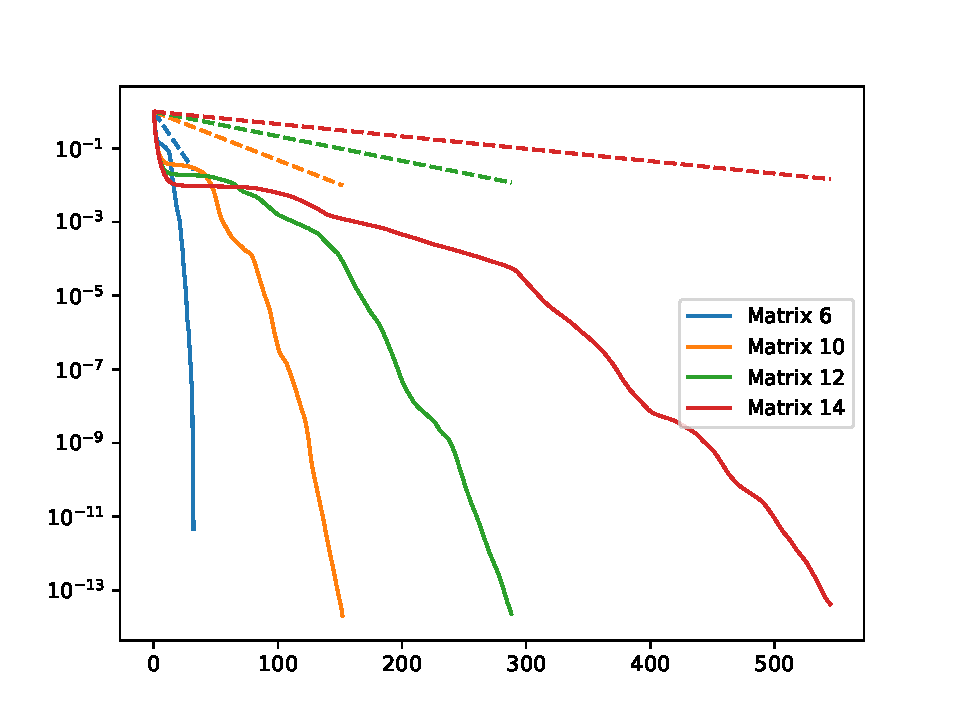
\includegraphics[height=5in]{Problem2-ErrorPlot-First4.pdf}

Next, since the condition numbers for the larger matrices were also determined, we can plot the
results for the larger matrices as well: \\
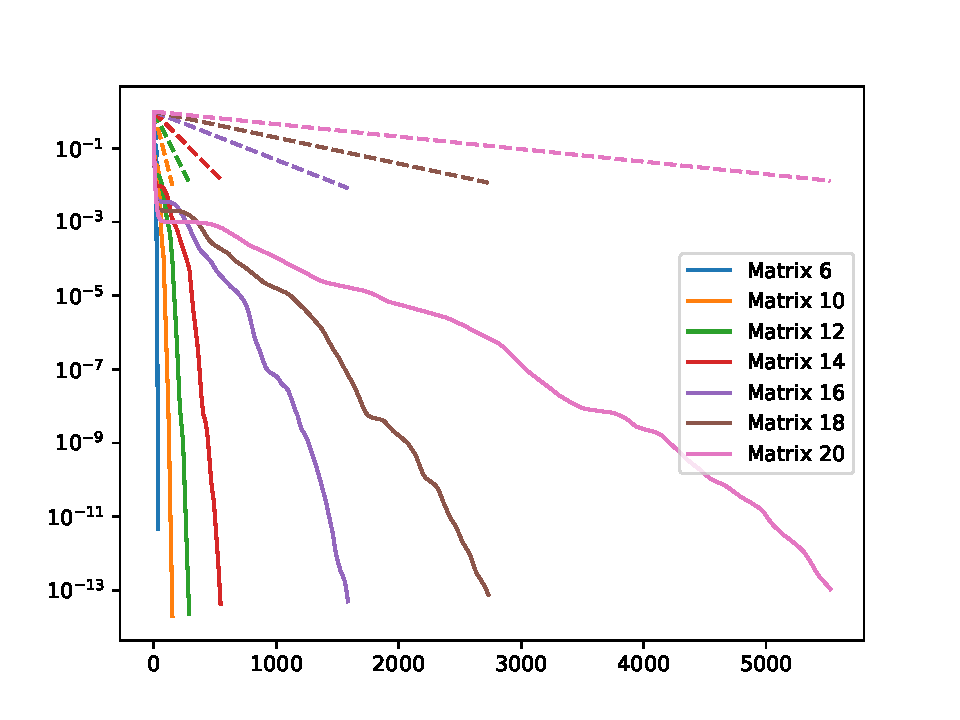
\includegraphics[height=5in]{Problem2-ErrorPlot-all.pdf}

In all cases, we do see that the error never exceeds the theoretical bound and especially for the
larger matrices, tends to be much lower.
\end{document}